\subsection{Linear Lagrangian Finite Element Space Base}

Given $\Omega = (0, 1)$ and $T_h$ a partition on $\Omega$, we'd have to define a base on $V_h$ which is, as discussed before, the linear Lagrangian finite element space on $T_h$.

Let $x_j$ a node for $T_h$, we define $\phi_j$ as it follows:
\begin{gather}
	\phi_j(x_i) = \delta_{ij}.
\end{gather}

Moreover, the functions $\phi_j(x)$ are continuos and piecewise linear, which satisfies $\phi_j(x) \in V_h$ $\forall j \in \{1, \dots, N_{V_h}\}$.

\subsection{Finite Element Discretization}
As seen on \nameref{fem_definition}, the finite element discretization consists in finding $u_h \in V_h$ such that:
\begin{gather}
	a(u_h, v_h) = (f, v_h)_{0, \Omega} \quad \forall v_h \in V_h.
\end{gather}

Consider $\{\phi_j\}_j$ base on $V_h$ so that we can write:
\begin{gather}
	u_h(x) = \sum_{j = 1}^{N_{V_h}} u_j \phi_j(x),
\end{gather}
where $N_{V_h} = \dim(V_h)$ and $\underline{u} \in \R^{N_{V_h}}$, so that it is sufficient considering:
\begin{gather}
	a(u_h, \phi_j) = (f, \phi_j)_{0, \Omega} \quad \forall j \in \{1, \dots, N_{V_h}\}.
\end{gather}

This lets us ultimately write the following linear system:
\begin{gather}
	\underline{\underline{A}} \underline{u} = \underline{f},
\end{gather}
where $A_{ij} = a(\phi_i, \phi_j)$, $f_i = (f, \phi_i)_{0, \Omega}$.

\subsection{FEM Convergence on Uniform Meshes}

Given what we've said on \nameref{sob_regularity}, and by the following corollary to the \textit{Deny-Lions' Lemma}:

\begin{theorem}[Deny-Lions corollary]
	Let $u, u_h$ be the solution respectively to the weak formulation of a Poisson problem and its associated order k Lagrangian FEM with shape-regular and quasi-uniform mesh $T_h$. \\ 
	If $u \in H^s(\Omega)$, then $\exists C$ such that:
	\begin{gather}
		|u - u_h|_{1, \Omega} \le C (\max_{K \in T_h} h_K)^{p}|u|_{s+1, \Omega},
	\end{gather}
	with $p = \min(s, k)$.
\end{theorem}

Having defined a 1st-order Lagrangian FEM, we have for both values of $\alpha$ that $p = 1$, so that\footnote{The value of $s$ depends on the value of $\alpha$. We can always choose $s > k$.}:
\begin{gather}
	|u - u_h|_{1, \Omega} \le C (\max_{K \in T_h} h_K)|u|_{s+1, \Omega}.
\end{gather}

By\footnote{For an appropriate choice of $s$.}:
\begin{gather}
	\max_{K \in T_h} h_K = h, \\
	|u|_{s+1, \Omega} < +\infty,
\end{gather}
we have:
\begin{gather}
	|u - u_h|_{1, \Omega} \le C_1 h.
\end{gather}

\begin{figure}[!ht]
	\centering
	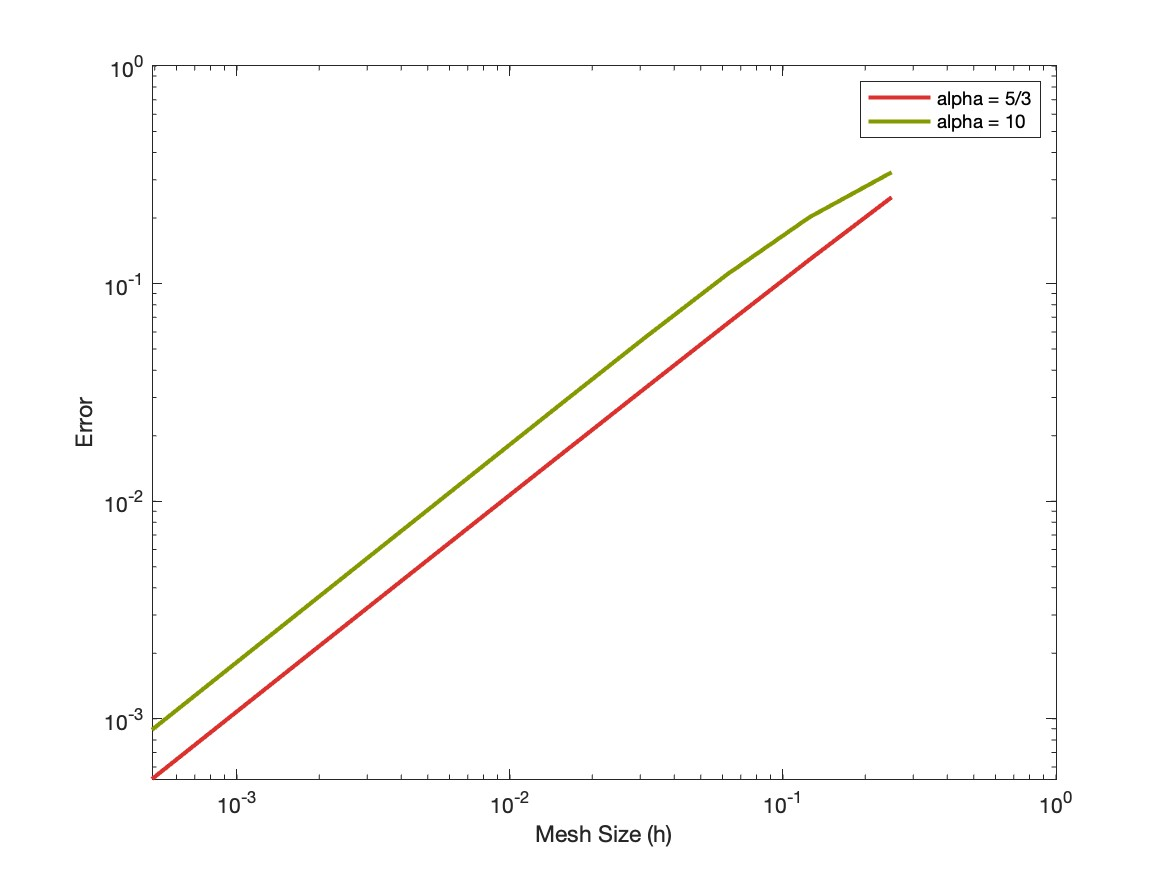
\includegraphics[width=15cm]{errorTrend.jpg}
	\caption{Error trend against mesh size for a sequence of uniform meshes.}
\end{figure}

\noindent Moreover a polynomial interpolation returns the following results which confirm the expected error trend on uniform meshes, as they are decreasing slightly slower than linearly.
\begin{verbatim}
alpha = 5/3, y = 0.988762x + (0.006448)
alpha = 10, y = 0.964138x + (0.389059)
\end{verbatim}